\textbf{See the instruction for questions \inteval{\value{question}+1} to \inteval{\value{question}+2}.}

\begin{figure}[H]
\centering
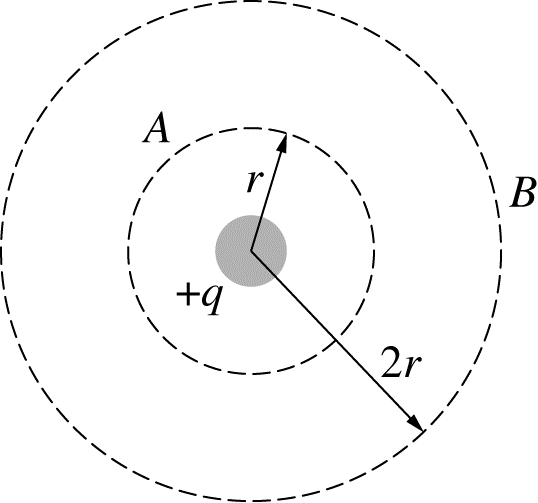
\includegraphics[scale=0.3]{images/img-003-001.png}
\end{figure}

A small sphere has a charge $+q$. Spherical Gaussian surfaces $A$ and $B$ are concentric with the sphere, as shown in the figure above. The radii of surfaces $A$ and $B$ are $r$ and $2r$, respectively.

% Multiple Choice Question 3
\begin{questions}\setcounter{question}{2}\question
The magnitude of the electric flux through $A$ is $\Phi_{A}$. The magnitude of the electric flux through surface $B$ is $\Phi_{B}$. The ratio $\Phi_{A} / \Phi_{B}$ is

\begin{oneparchoices}
\choice $4 / 1$
\choice $2 / 1$
\choice $1 / 1$
\choice $1 / 2$
\choice $1 / 4$
\end{oneparchoices}\end{questions}

% Multiple Choice Question 4
\begin{questions}\setcounter{question}{3}\question
The magnitude of the electric field at surface $A$ is $E_{A}$. The magnitude of the electric field at surface $B$ is $E_{B}$. The ratio $E_{A} / E_{B}$ is

\begin{oneparchoices}
\choice $4 / 1$
\choice $2 / 1$
\choice $1 / 1$
\choice $1 / 2$
\choice $1 / 4$
\end{oneparchoices}\end{questions}
